%KDD% \vspace{-1mm}
\section{Comparison of NLP Models}
\label{sxn:nlp}
%\vspace{-1mm}

In this section, we examine empirical quality metrics described in Section~\ref{sxn:methods} for several NLP model architectures.
%
%In particular, 
Within the past two years, nearly 100 open source, pretrained NLP DNNs based on the revolutionary Transformer architecture have emerged.
These include variants of BERT, Transformer-XML, GPT, etc.
%
The Transformer architectures consist of blocks of so-called Attention layers, containing two large, Feed Forward (Linear) weight matrics~\cite{Attn2017}. 
In contrast to smaller pre-Activation maps arising in Cond2D layers, Attention matrices are significantly larger.
In general, we have found that they have larger PL exponents $\alpha$.
Based on HT-SR Theory, 
%(in particular, the interpretation of values of $\alpha \sim 2$ as modeling systems with good correations over many size scales~\cite{BouchaudPotters03, SornetteBook}), 
this suggests that these models fail to capture successfully many of the correlations in the data (relative to their size) and thus are substantially \emph{under}-trained.
%
More generally, compared to the CV models of Section~\ref{sxn:cv},
modern NLP models have larger weight matrices and display different spectral properties.
%, both in terms of their architecture (e.g., wheter there are convolutions) as well as how they are used (e.g., whether one uses prediction error or perplexity).
Thus, they provide a very different test for our empirical quality metrics.

While norm-based metrics perform reasonably well on well-trained NLP models, they often behave anomalously on poorly-trained models.
Indeed, for such ``bad'' models, weight matrics may display rank collapse, decreased Frobeinus mass, or unsually small Spectral norms.
(This may be misinterpreted as ``smaller is better.'')
In contrast, PL-based metrics, including the Log $\alpha$-Norm metric ($\log\Vert\mathbf{W}\Vert_{\alpha}^{\alpha}$) and the Weighted Alpha metric ($\hat\alpha =\alpha\log\lambda_{max} $) display consistant behavior, even on poorly trained models.
Indeed, we can use these metrics to help indentify when archiectures need repair and when more and/or better data are needed.


%KDD% \vspace{-1mm}
\paragraph{What do large values of $\alpha$ mean?}

Many NLP models, such as GPT and BERT, have some weight matrices with unusually large PL exponents (e.g., $\alpha\gg 6$).
This indicates these matrices may be \emph{under}-correlated (i.e., over-parameterized, relative to the amount of data).
In this regime, the truncated PL fit itself may not be very reliable because the MLE estimator it uses is unreliable in this range (i.e., the specific $\alpha$ values returned by the truncated PL fits are less reliable, but having large versus small values of $\alpha$ is reliable).
Phenomenologically, if we examine the ESD visually, we can usually describe these $\mathbf{W}$ as in the \emph{Bulk-Decay} or \emph{Bulk-plus-Spikes} phase~\cite{MM18_TR,MM19_HTSR_ICML}.
Previous work~\cite{MM18_TR,MM19_HTSR_ICML} has conjectured that very well-trained DNNs would not have many \emph{outlier} $\alpha>6$; and improved versions of GPT (shown below) and BERT (not shown) confirm this.


%KDD% \vspace{-1mm}
\paragraph{OpenAI GPT Models.}

The OpenAI GPT and GPT2 models provide us with the opportunity to analyze two effects: training the same model with different data set sizes; and increasing the sizes of both the data set and the architectures simultaneously.
These models have the remarkable ability to generate fake text that appears to the human to be real, and they have generated significant media attention because of the potential for their misuse.
For this reason, the original GPT model released by OpenAI was trained on a deficient data set, rendering the model interesting but not fully functional.  
Later, OpenAI released a much improved model, GPT2-small, which has the same architecture and number of layers as GPT, but which has been trained on a larger and better data set (and with other changes), making it remarkably good at generating (near) human-quality fake text.  
%
By comparing the poorly-trained (i.e., ``bad'') GPT to the well-trained (i.e., ``good'') GPT2, we can indentify empirical indidcators for when a model has in fact been poorly-trained and thus may perform poorly when deployed.
By comparing GPT2-medium to GPT2-large to GPT2-xl, we can examine the effect of increasing data set and model size simultaneously.

The GPT models we analyze are deployed with the popular HuggingFace PyTorch library~\cite{huggingface}.
GPT has 12 layers, with 4 Multi-head Attention Blocks, giving $48$ layer Weight Matrices, $\mathbf{W}$.
Each Block has 2 components, the Self Attention (attn) and the Projection (proj) matrics.  
The self-attention  matrices are larger, of dimension ($2304\times 768$) or ($3072\times 768$).
The projection layer concatenates the self-attention results into a vector (of dimension $768$).
This gives $50$ large matrices.
%
Because GPT and GPT2 are trained on different data sets, the initial Embedding matrices differ in shape.
GPT has an initial Token and Positional Embedding layers, of dimension $(40478\times 768)$ and $(512\times 768)$, respectively, whereas GPT2 has input Embeddings of shape $(50257\times 768)$ and $(1024\times 768)$, respectively. 
%
The OpenAI GPT2 (English) models are: GPT2-small, GPT2-medium, GPT2-large, and GPT2-xl, having $12, 24, 36, \text{and } 48$ layers, respectively, with increasingly larger weight matrices.
%The model card for GPT2 is published on github.\footnote{\url{https://github.com/openai/gpt-2/blob/master/model_card.md}}.


\begin{table}[t]
\small
\begin{center}
\begin{tabular}{|p{1in}|c|c|c|c|c|}
%KDD% \begin{tabular}{|p{0.67in}|c|c|c|c|c|}
\hline
 Series  & \#   & $\langle\log\Vert\mathbf{W}\Vert_{F}\rangle$ & $\langle\log\Vert\mathbf{W}\Vert_{\infty}\rangle$ & $\hat{\alpha}$ & $\langle\log\Vert\mathbf{X}\Vert^{\alpha}_{\alpha}\rangle$ \\
\hline
GPT & 49 & 1.64  & 1.72 & 7.01 & 7.28 \\
GPT2-small & 49 & 2.04  & 2.54& 9.62 & 9.87 \\
\hline
GPT2-medium & 98 & 2.08 & 2.58& 9.74 & 10.01 \\
GPT2-large & 146 & 1.85 & 1.99& 7.67 & 7.94 \\
GPT2-xl & 194 & 1.86 & 1.92 & 7.17 & 7.51 \\
\hline
\end{tabular}
\end{center}
\caption{Average value for the average Log Norm and Weighted Alpha metrics for pretrainnd OpenAI GPT and GPT2 models. Column \# refers to number of layers treated.  Note that the averages do not include the first embedding layer(s) because they are not (implicitly) normalized.  }
\label{table:nlp}
\end{table}


%KDD% \vspace{-1mm}
\paragraph{Average Quality Metrics for GPT and GPT2.}

We have analyzed the four quality metrics described in Section~\ref{sxn:methods} for the OpenAI GPT and GPT2 pretrained models.
See Table \ref{table:nlp} for a summary of results.
We start by examining trends between GPT and GPT2-small.
Observe that all four metrics increase when going from GPT to GPT2-small, i.e., they are smaller for the higher-quality model (higher quality since GPT was trained to better data), when the number of layers is held fixed.
Notice that in the GPT model, being poorly trained, the norm metrics all exhibit \emph{Scale Collapse}, compared to GPT2-small.

We next examine trends between GPT2-medium to GPT2-large to GPT2-xl.
Observe that (with one minor exception involving the log Frobenius norm metric) all four metrics decrease as one goes from medium to large to xl, indicating that the larger models indeed look better than the smaller models.
Notice that, for these well-trained models, the norm metrics now behave as expected, decreasing with increasing accuracy.

Going beyond average values, Figure~\ref{fig:GPT-alpha-hist} shows the histogram (empirical density), for all layers, of $\alpha$ for GPT and GPT2-small.  
These two histograms are very different.
The older deficient GPT has numerous unsually large $\alpha$ exponents---meaning they are not really well-described by a PL fit.
Indeed, we expect that a poorly-trained model will lack good (i.e., small $\alpha$) PL behavior in many/most layers.
On the other hand, as expected, the newer improved GPT2-small model has, on average, smaller $\alpha$ values than the older GPT, with all $\alpha\le6$ and with smaller mean/median $\alpha$, and it also has far fewer unusually-large outlying $\alpha$ values than GPT.
From this (and other results not shown), we see that $\alpha$ provides a good quality metric for comparing these two models, the ``bad'' GPT versus the ``good'' GPT2-small.
%
This should be contrasted with the behavior displayed by the Frobenius norm (not shown) and the Spectral~norm.


%KDD% \vspace{-1mm}
\paragraph{Scale Collapse in Poorly Trained Models.}

We next describe the behavior of the Spectral norm in GPT versus GPT2-small.
In Figure~\ref{fig:GPT-snorm-hist}, the ``bad'' GPT model has a smaller mean/median Spectral norm as well as, spuriously, many much smaller Spectral norms, compared to the ``good'' GPT2-small, violating the conventional wisdom that smaller Spectral norms are better.
Indeed, because there are so many anonymously small Spectral norms, it appears that the GPT model may be exhibiting a kind of \emph{Scale Collapse}, like that observed in the distilled CV models (in Figure~\ref{fig:resnet204D5L}).
This is important because it demonstrates that, while the Spectral norm may correlate well with predicted test error, it is \emph{not} a good indicator of the overall model quality.
It can mispredict good-versus-bad questions in ways not seen with PL-based metrics.
Using it as an empirical quality metric may give spurious results when applied to poorly-trained or otherwise deficient models. 

\begin{figure}[h]
    \centering
    \subfigure[PL exponent ($\alpha$)]{
        %KDD% 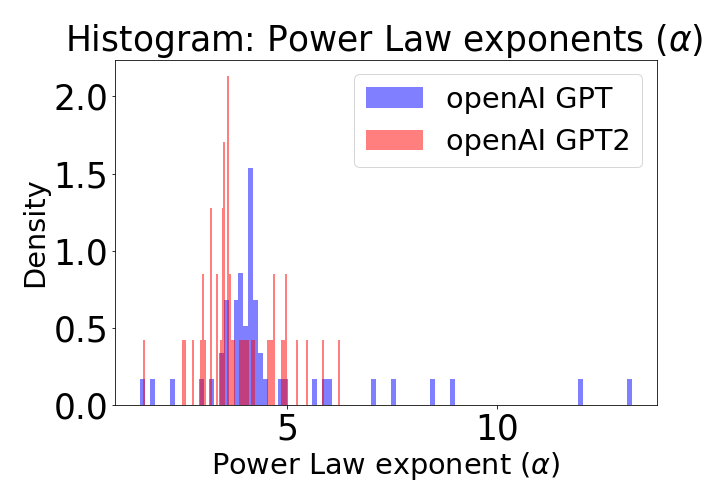
\includegraphics[width=4.0cm]{img/GPT-alpha-hist.png}
        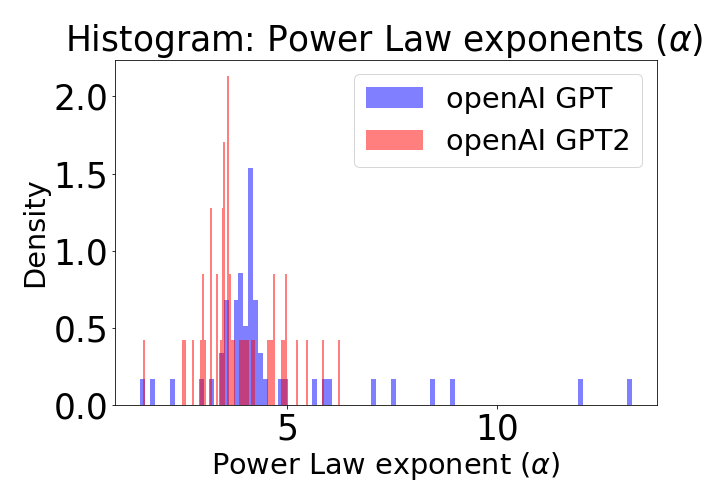
\includegraphics[width=5.5cm]{img/GPT-alpha-hist.png}
        \label{fig:GPT-alpha-hist}
       }
    %KDD% 
    \qquad
    \subfigure[Log Spectral Norm ($\log\Vert\mathbf{W}\Vert_{\infty}$)]{
        %KDD% 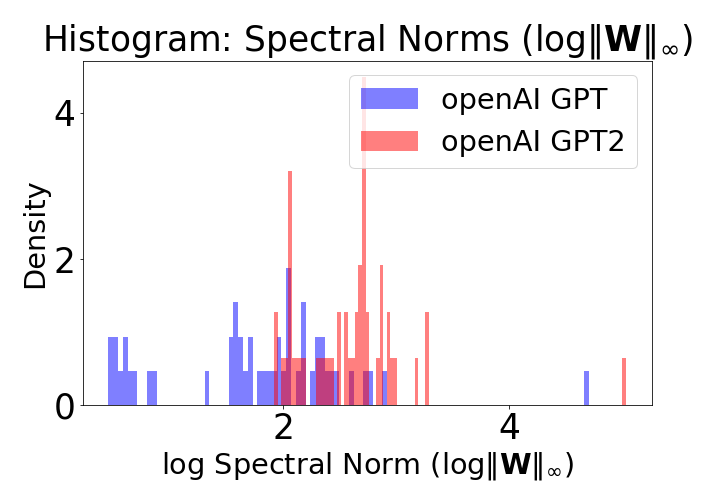
\includegraphics[width=4.0cm]{img/GPT-snorm-hist.png}
        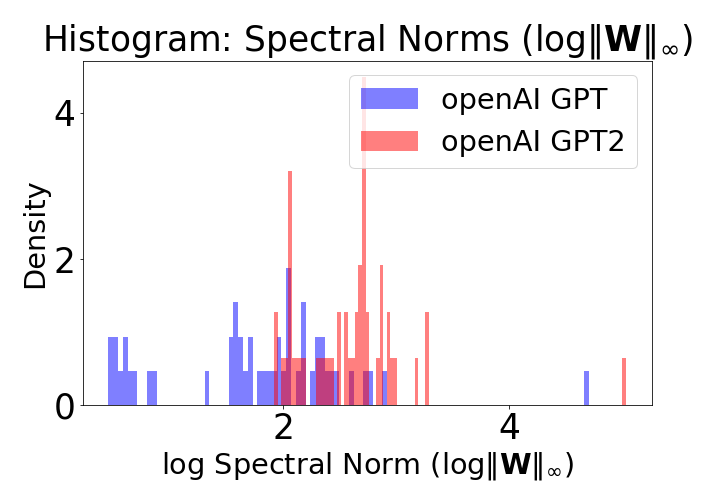
\includegraphics[width=5.5cm]{img/GPT-snorm-hist.png}
        \label{fig:GPT-snorm-hist}
       }
   \caption{Histogram of PL exponents ($\alpha$) and Log Spectral Norms ($\log\Vert\mathbf{W}\Vert_{\infty}$) for weight matrices from the OpenAI GPT and GPT2-small pretrained models.}
   
\label{fig:GPT-hist}
\end{figure}


Note that Figure~\ref{fig:GPT-snorm-hist} also shows some unusually large Spectral Norms.
Upon examination, e.g., from Figure \ref{fig:gpt-snorm-layer} (below), we see that these correspond to the first embedding layer(s).
%That is, they correspond to the change in normalization of the word embedding layer(s), and thus they can be ignored.
These layers have a different effective normalization, and therefore a different scale.
% \charles{We discuss this further in Appendix~\ref{sxn:appendix}.}
% For example, in GPT, for most layers, the maximum eigenvalue $\lambda_{max}\sim\mathcal{O}(10-100)$, but in the first embedding layer, the maximum is of order $N$ (the number of words in the embedding), or $\lambda_{max}\sim\mathcal{O}(10^{5})$.  
% For GPT and GPT2, we treat all layers as-is (although one may want to normalize the first 2 layers by $\mathbf{X}$ by $1/N$ or treat them as an outlier).
We discuss this further in Appendix~\ref{sxn:appendix}.
Here, we do not include them in our computed average metrics in Table~\ref{table:nlp}, and we do not include them in the histogram plot in Figure~\ref{fig:GPT-snorm-hist}.



%KDD% \vspace{-1mm}
\paragraph{Layer Analysis: Correlation Flow and Scale Collapse in GPT and GPT2.} 

We also examine in Figure~\ref{fig:gpt-alpha-layers} the PL exponent $\alpha$ and Log Spectral Norm versus layer id, for GPT and GPT2-small.
Let's start with Figure~\ref{fig:gpt-alpha-layer}, which plots $\alpha$ versus the depth (i.e., layer id) for each model.
The deficient GPT model displays two trends in $\alpha$, one stable with $\alpha\sim 4$, and one increasing with layer id, with $\alpha$ reaching as high as $12$.
In contrast, the well-trained GPT2-small model shows consistant and stable patterns, again with one stable $\alpha\sim 3.5$ (and below the GPT trend), and the other only slightly trending up, with $\alpha\le 6$. 
The scale-invariant $\alpha$ metric lets us identify potentially poorly-trained models; and these results show that the Correlation Flow differs significantly between GPT and GPT2-small (with the better GPT2-small looking more like the better ResNet-1K from Figure~\ref{fig:resnet-alpha-layer}).

These results should be contrasted with the corresponding results for Spectral Norms, shown in Figure~\ref{fig:gpt-snorm-layer}.
Attention models have two types of layers, one small and large; and the Spectral Norm, in particular, displays unusually small values for some of these layers for GPT.
This Scale Collapse for the poorly-trained GPT is similar to what we observed for the distilled ResNet20 model in Figure~\ref{fig:resnet204Dalpha}.
Because of the anomalous scale collapse that is frequently observed in poorly-trained models, these results suggest that scale-dependent norm metrics should not be directly applied to distinguish good-versus-bad models. 


\begin{figure}[htb]
    \centering
    \subfigure[PL exponent ($\alpha$)]{
        %KDD% 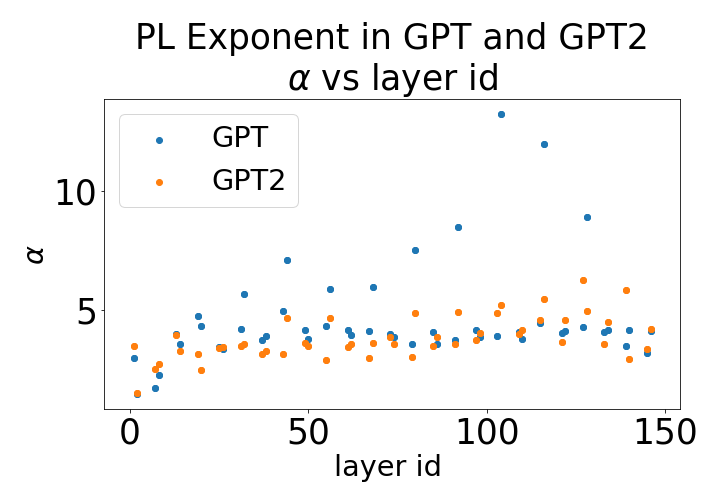
\includegraphics[width=4.0cm]{img/GPT-alpha-depth.png}
        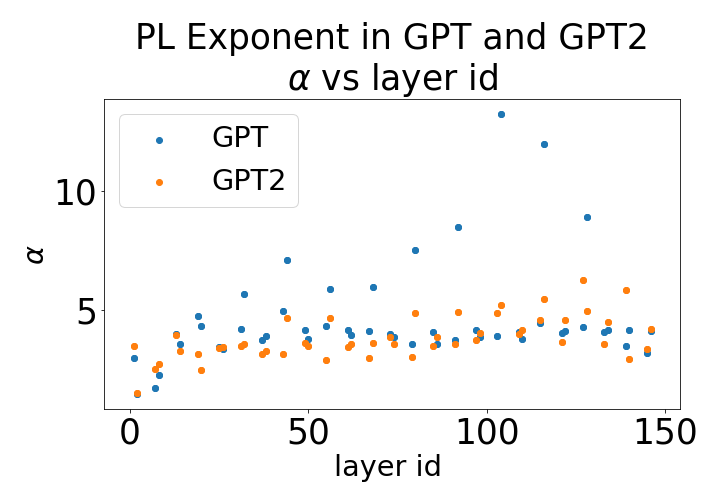
\includegraphics[width=5.5cm]{img/GPT-alpha-depth.png}
        \label{fig:gpt-alpha-layer}
    }
    %KDD% 
    \quad
    \subfigure[Log Spectral Norm ($\log\Vert\mathbf{W}\Vert_{\infty}$)]{
        %KDD% 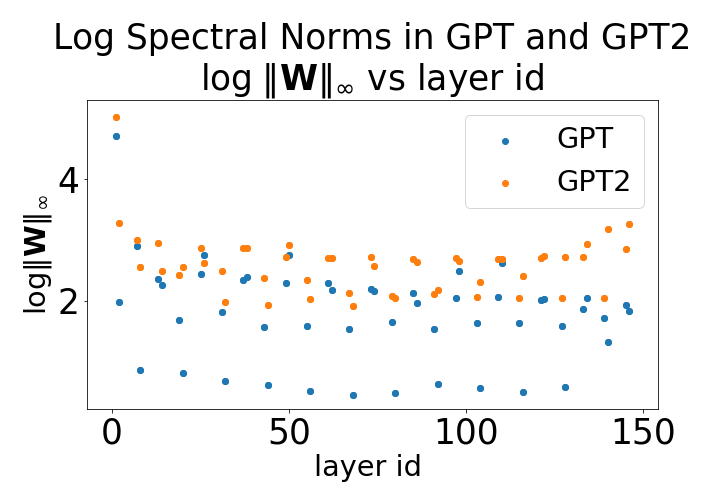
\includegraphics[width=4.0cm]{img/GPT-snorm-depth.png}
        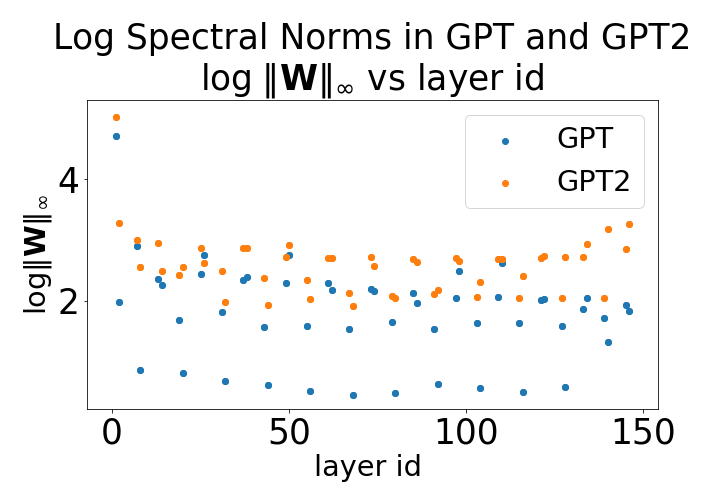
\includegraphics[width=5.5cm]{img/GPT-snorm-depth.png}
        \label{fig:gpt-snorm-layer}
    }
    \caption{PL exponents ($\alpha$) (in (a)) and Log Spectral Norms ($\log\Vert\mathbf{W}\Vert_{\infty}$) (in (b)) for weight matrices from the OpenAI GPT and GPT2-small pretrained models.  (Note that the Y axes on each plot are different.)
             In the text, this is interpreted in terms of \emph{Correlation Flow} and \emph{Scale~Collapse}.
            }
    \label{fig:gpt-alpha-layers}
\end{figure}


%KDD% \vspace{-1mm}
\paragraph{GPT2: medium, large, xl.} 

We now look across series of increasingly improving GPT2 models (i.e., we consider good-better-best questions), by examining both the PL exponent $\alpha$ as well as the Log Norm metrics.  
In general, as we move from GPT2-medium to GPT2-xl, histograms for both $\alpha$ exponents and the Log Norm metrics downshift from larger to smaller values. 
For example, see Figure \ref{fig:gpt2-histograms}, which shows the histograms over the layer weight matrics for fitted PL exponent ($\alpha$) and the Log Alpha Norm ($\log\Vert\mathbf{W}\Vert_{\alpha}^{\alpha}$)~metric.

We see that the average $\alpha$ decreases with increasing model size, although the differences are less noticible between the differing good-better-best GTP2 models than between the good-versus-bad GPT and GPT2-small models.
Unlike GPT, however, the layer Log Alpha Norms behave more as expected for GPT2 layers, with the larger models consistently having smaller norms. 
Similarly, the Log Spectral Norm also decreases on average with the larger models (not shown).  
As expected, the norm metrics can indeed distinguish among good-better-best models among a series well-trained models.

We do notice, however, that while the peaks of the $\alpha$ are getting smaller, towards $2.0$, the tails of the distribution shifts right, with larger GPT2 models having more usually large $\alpha$ (also not shown).  
We suspect this indicates that these larger GPT2 models are still under-optimized/over-parameterized (relative to the data on which they were trained) and that they have capacity to support datasets even larger than the recent XL $1.5B$ release~\cite{gpt2-xl}.

\begin{figure}[htb]
    \centering

    \subfigure[PL exponent ($\alpha$)]{
        %KDD% 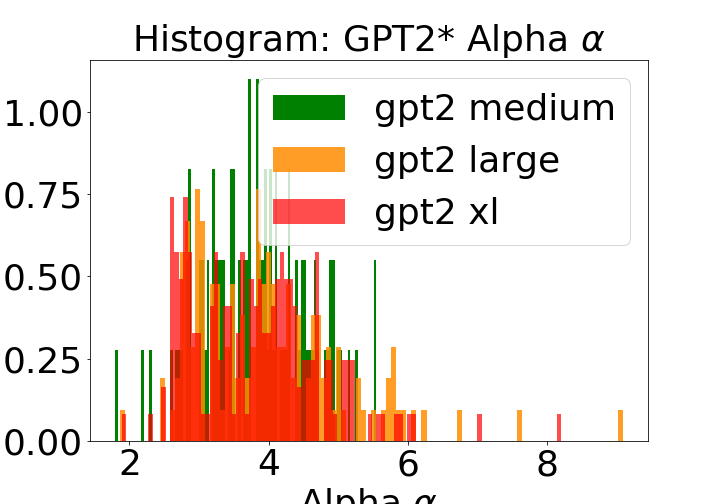
\includegraphics[width=4.0cm]{img/GPT2*_fnl_alpha_hist.png}
        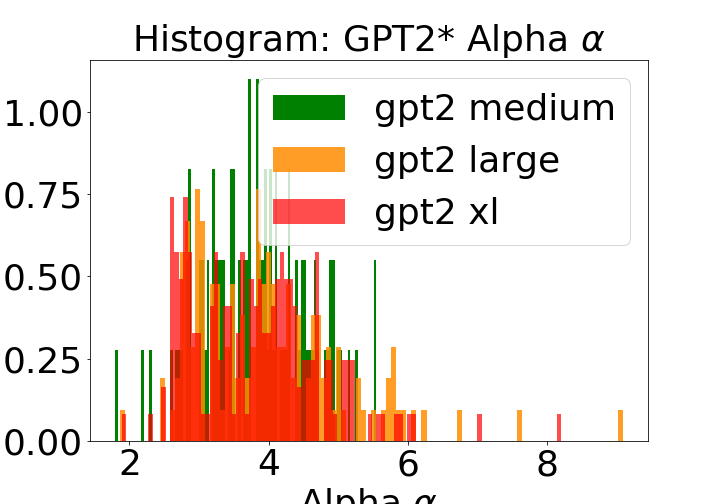
\includegraphics[width=5.5cm]{img/GPT2*_fnl_alpha_hist.png}
        \label{fig:gpt2-alpha-hist}
    }
    %KDD% 
    \quad
    \subfigure[Log Alpha Norm]{
        %KDD% 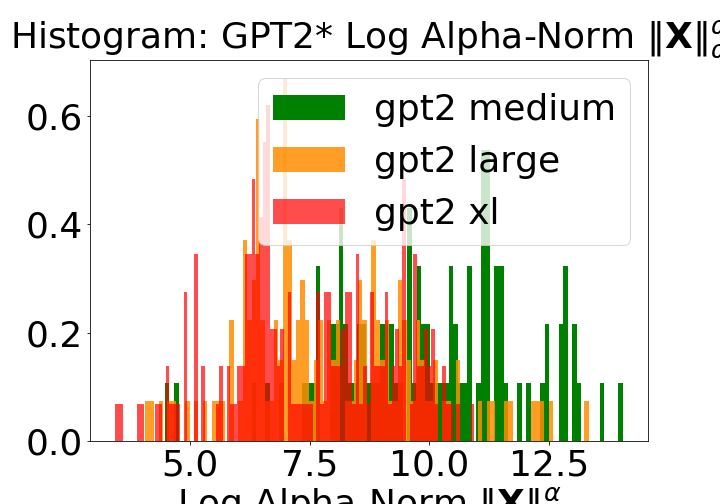
\includegraphics[width=4.0cm]{img/GPT2*_fnl_logpnorm_hist.png}
        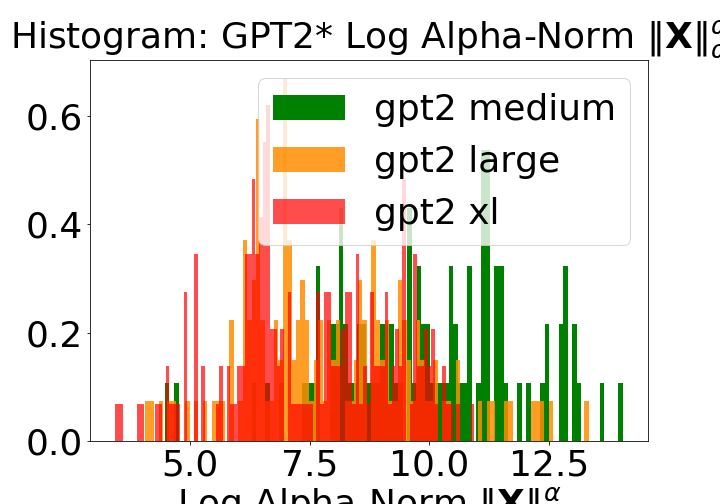
\includegraphics[width=5.5cm]{img/GPT2*_fnl_logpnorm_hist.png}
        \label{fig:gpt2-pnorm-hist}
    }
    \caption{Histogram of PL exponents ($\alpha$)
             %Log Spectral norm ($\log\Vert\mathbf{W}\Vert_{\infty}$), 
              and Log Alpha Norm ($\log\Vert\mathbf{X}\Vert_{\alpha}^{\alpha}$) for weight matrices from models of different sizes in the GPT2 architecture series.  (Plots omit the first 2 (embedding) layers, because they are normalized differently giving anamolously large values.)
             }
    \label{fig:gpt2-histograms}
\end{figure}
